\apendice
\chapter{Tabela de Comparação entre as Soluções Analisadas} \label{apendiceA}
%%%====== INICIO TABELA ======%%%
\begin{landscape}
\fontsize{8.5}{12}\selectfont
\tabcolsep=0.11cm
\begin{longtable}[c]{c|p{.09\textwidth}|p{.07\textwidth}|p{.065\textwidth}|p{.102\textwidth}|p{.10\textwidth}|p{.10\textwidth}|p{.10\textwidth}|p{.10\textwidth}|p{.09\textwidth}|p{.085\textwidth}|p{.10\textwidth}|p{.06\textwidth}|p{.06\textwidth}|p{.10\textwidth}|p{.07\textwidth}|p{.08\textwidth}|p{.06\textwidth}}
\caption{Comparação entre as Soluções, forma comercial e acadêmica}
\label{comparacaoCriterios}\\
\hline
\multicolumn{2}{c|}{\multirow{3}{*}{CRITÉRIOS}} & \multicolumn{16}{c}{SOLUÇÕES} \\ \cline{3-18} 
\multicolumn{2}{c|}{} & \multicolumn{9}{c|}{COMERCIAL} & \multicolumn{7}{c}{ACADÊMICO} \\ \cline{3-18} 
\multicolumn{2}{c|}{} & MusicID & Shazam & SoundHound & Deezer & Spotify & SoundCloud & Musixmatch & ACRCloud & Musipedia & MusicMiner & YALE & CLAM & MIRtoolbox & AMUSE & Java MIR & Tunebot \\ \hline
\endfirsthead
%
\multicolumn{18}{c}%
{{\bfseries \tablename\ \thetable\ continuação da página anterior}} \\
\hline
\multicolumn{2}{c|}{\multirow{3}{*}{CRITÉRIOS}} & \multicolumn{16}{c}{SOLUÇÕES} \\ \cline{3-18} 
\multicolumn{2}{c|}{} & \multicolumn{9}{c|}{COMERCIAL} & \multicolumn{7}{c}{ACADÊMICO} \\ \cline{3-18} 
\multicolumn{2}{c|}{} & MusicID & Shazam & SoundHound & Deezer & Spotify & SoundCloud & Musixmatch & ACRCloud & Musipedia & MusicMiner & YALE & CLAM & MIRtoolbox & AMUSE & Java MIR & Tunebot \\ \hline
\endhead
%
\multirow{3}{*}{\rotatebox[origin=c]{90}{Eficiência de desempenho}} & Comporta-mento em relação ao tempo & até 8s & até 8s & até 5s & até 10s & até 30s & até 30s & até 13s & até 5s & - & - & - & - & - & - & - & - \\ \cline{2-18} 
 & Utilização de recursos & FP & FP & IA & RPC e FP & RPC & RPC & RPC e FP & FP & Diversas & Diversas & - & SMS & Diversas & C & C e ML & QBH \\ \cline{2-18} 
 & Bitrate & até 128kbps & - & - & até 320kbps & até 320kbps & até 128kbps & - & - & - & - & - & - & - & - & - & - \\ \hline
\multirow{7}{*}{\rotatebox[origin=c]{90}{Adequação Funcional}} & Disponibi-lidade & iOS, Android & iOS, Android & iOS, Android & iOS, Android, Windows, Web, Roku TV & Linux, Windows, OS X, iOS, Android, Web & iOS, Android & iOS, Android & Web & Web & Linux, Mac OSX, Windows & - & Linux, Mac OSX, Windows & Linux, Mac OSX, Windows & - & Linux, Mac OSX, Windows & iOS \\ \cline{2-18} 
 & Modelo de desenvolvimento & F & F & F & F & F & F & F & F & A & A & - & A & A & A & F & F \\ \cline{2-18} 
 & Integrações & não & Spotify, Google Play Music, Apple Music & Twitter, Youtube, Spotify & não & não & não & Spotify, Google Play Music, Deezer, Youtube & ISRC, UPC, Spotify, Deezer, Youtube, LyricFind, Music Story e SyncPower & não & não & Music-Miner, AMU-SE & não & não & MIRtoolbox & não & Karaoke Callout \\ \cline{2-18} 
 & Acessibi-lidade & On & On & On & On/Off & On/Off & On & On & On & On & Off & - & Off & Off & Off & Off & On?/Off \\ \cline{2-18} 
 & Busca de dados & aprox. & exato & aprox. & exato & exato & exato & aprox. & aprox. & aprox. & aprox. & aprox. & aprox. & aprox. & aprox. & aprox. & aprox. \\ \cline{2-18} 
 & Inclusão de dados & não & não & não & não & não & sim & não & sim & sim & sim & sim & sim & sim & sim & sim & sim \\ \cline{2-18} 
 & Modelo de pagamento & G & G & F & F & F & F & F & P & G & G & - & G & G & G & G & G \\ \hline
\multirow{5}{*}{\rotatebox[origin=c]{90}{Usabilidade}} & Visibilida-de do status do sistema & sim & sim & sim & sim & sim & sim & sim & sim & sim & - & - & - & - & - & - & - \\ \cline{2-18} 
 & Prevenção de erros & sim & sim & sim & sim & sim & sim & sim & sim & não & - & - & - & - & - & - & - \\ \cline{2-18} 
 & Flexibili-dade e eficiência de uso & sim & sim & sim & sim & sim & sim & sim & sim & sim & - & - & - & - & - & - & - \\ \cline{2-18} 
 & Estética e Design minimalista & sim & sim & sim & sim & sim & sim & sim & sim & não & - & - & - & - & - & - & - \\ \cline{2-18} 
 & Pouca interação homem / dispositivo & sim & sim & sim & sim & sim & sim & sim & sim & sim & - & - & - & - & - & - & - \\ \hline
\caption*{Legenda: FP - FingerPrint; IA - Inteligência Artificial; RPC - Recuperação por Conteúdo; SMS - Spectral Modeling Synthesis; C - Classificação; QBH - Query by Humming; A - Aberto; F - Fechado; G - Gratuito; F - Freemium; P - Premium}
\end{longtable}
\end{landscape}
%%%====== FIM TABELA ======%%%


\chapter{Figuras} \label{apendiceB}
\begin{figure}[!htb]
   \centering
   \caption{MusicMiner}\label{fig:musicminer} 
   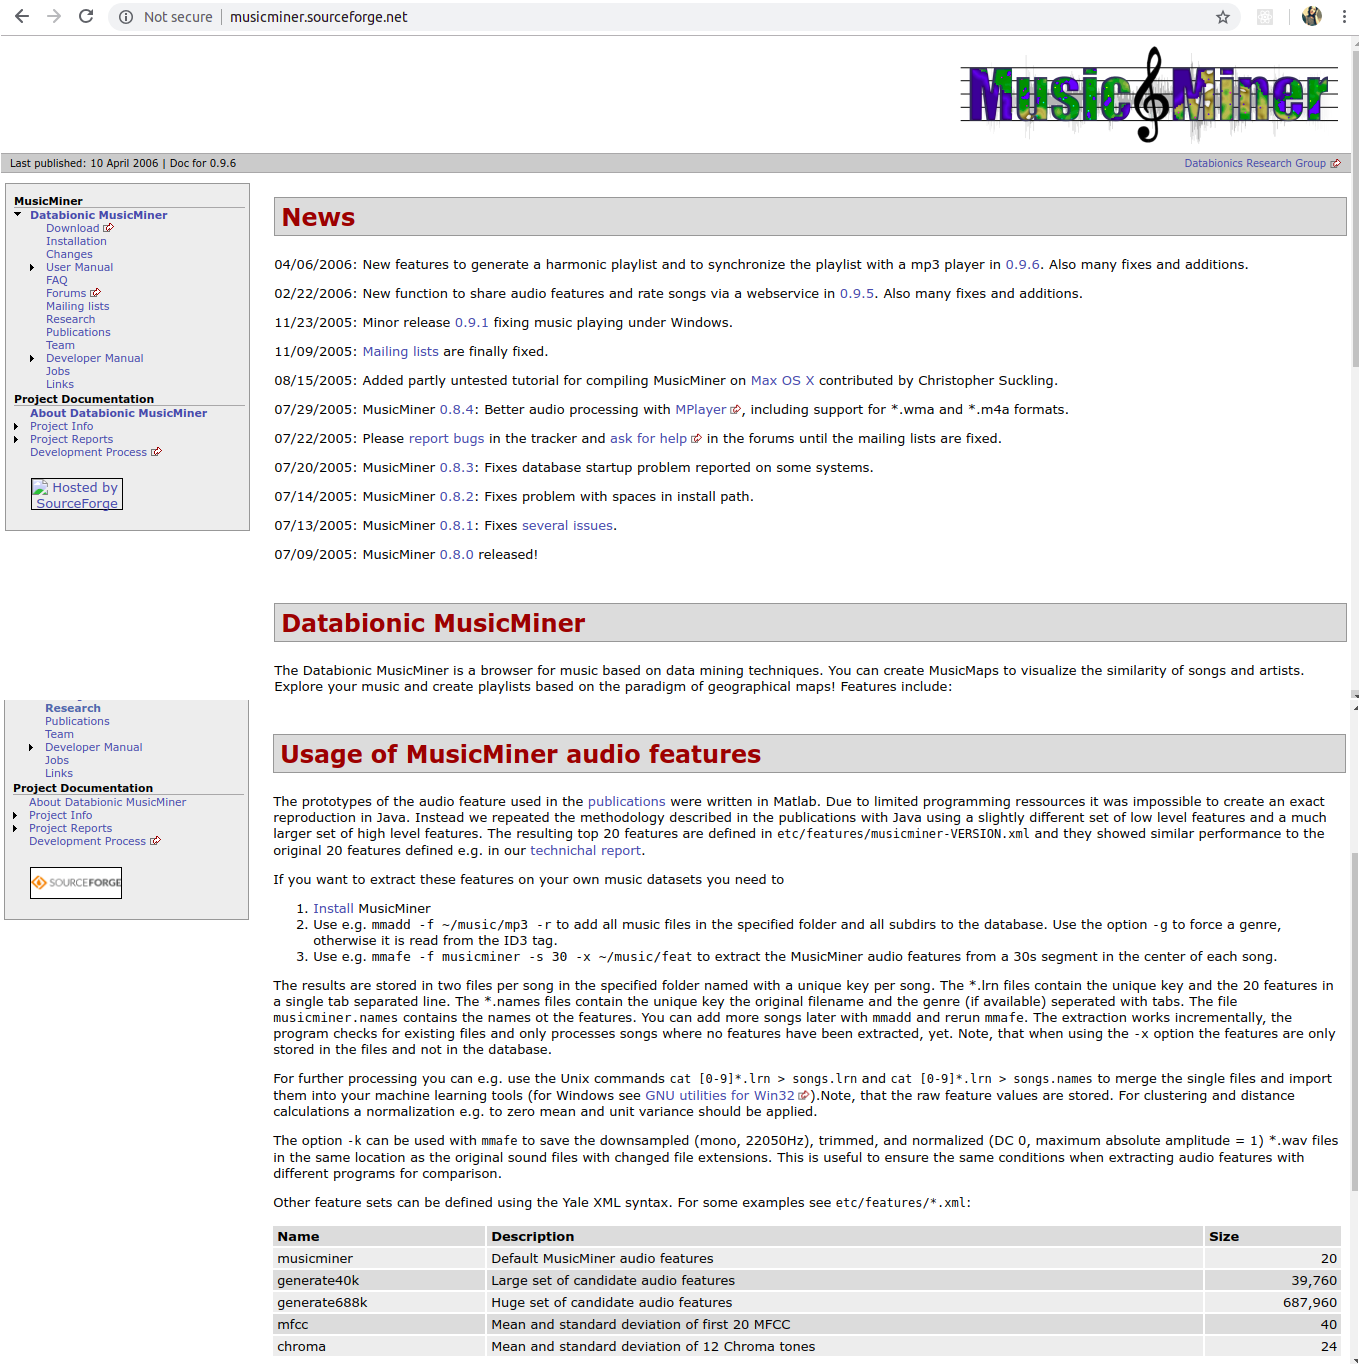
\includegraphics[scale=0.30]{figuras/musicminer.png}
   \\Fonte: \cite{musicminer}, elaborado pela autora
\end{figure}

\begin{figure}[!htb]
   \centering
   \caption{AMUSE}\label{fig:amuse} 
   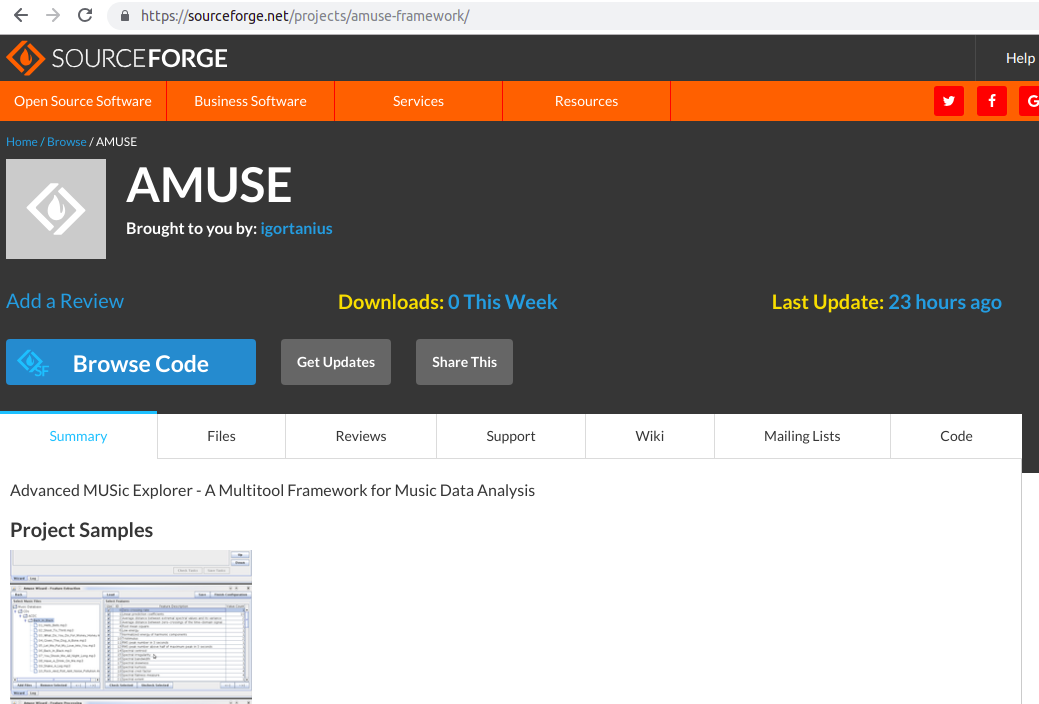
\includegraphics[scale=0.40]{figuras/amuse.png}
   \\Fonte: \cite{amuse}, elaborado pela autora
\end{figure}

\begin{figure}[!htb]
   \centering
   \caption{Java MIR}\label{fig:jmir} 
   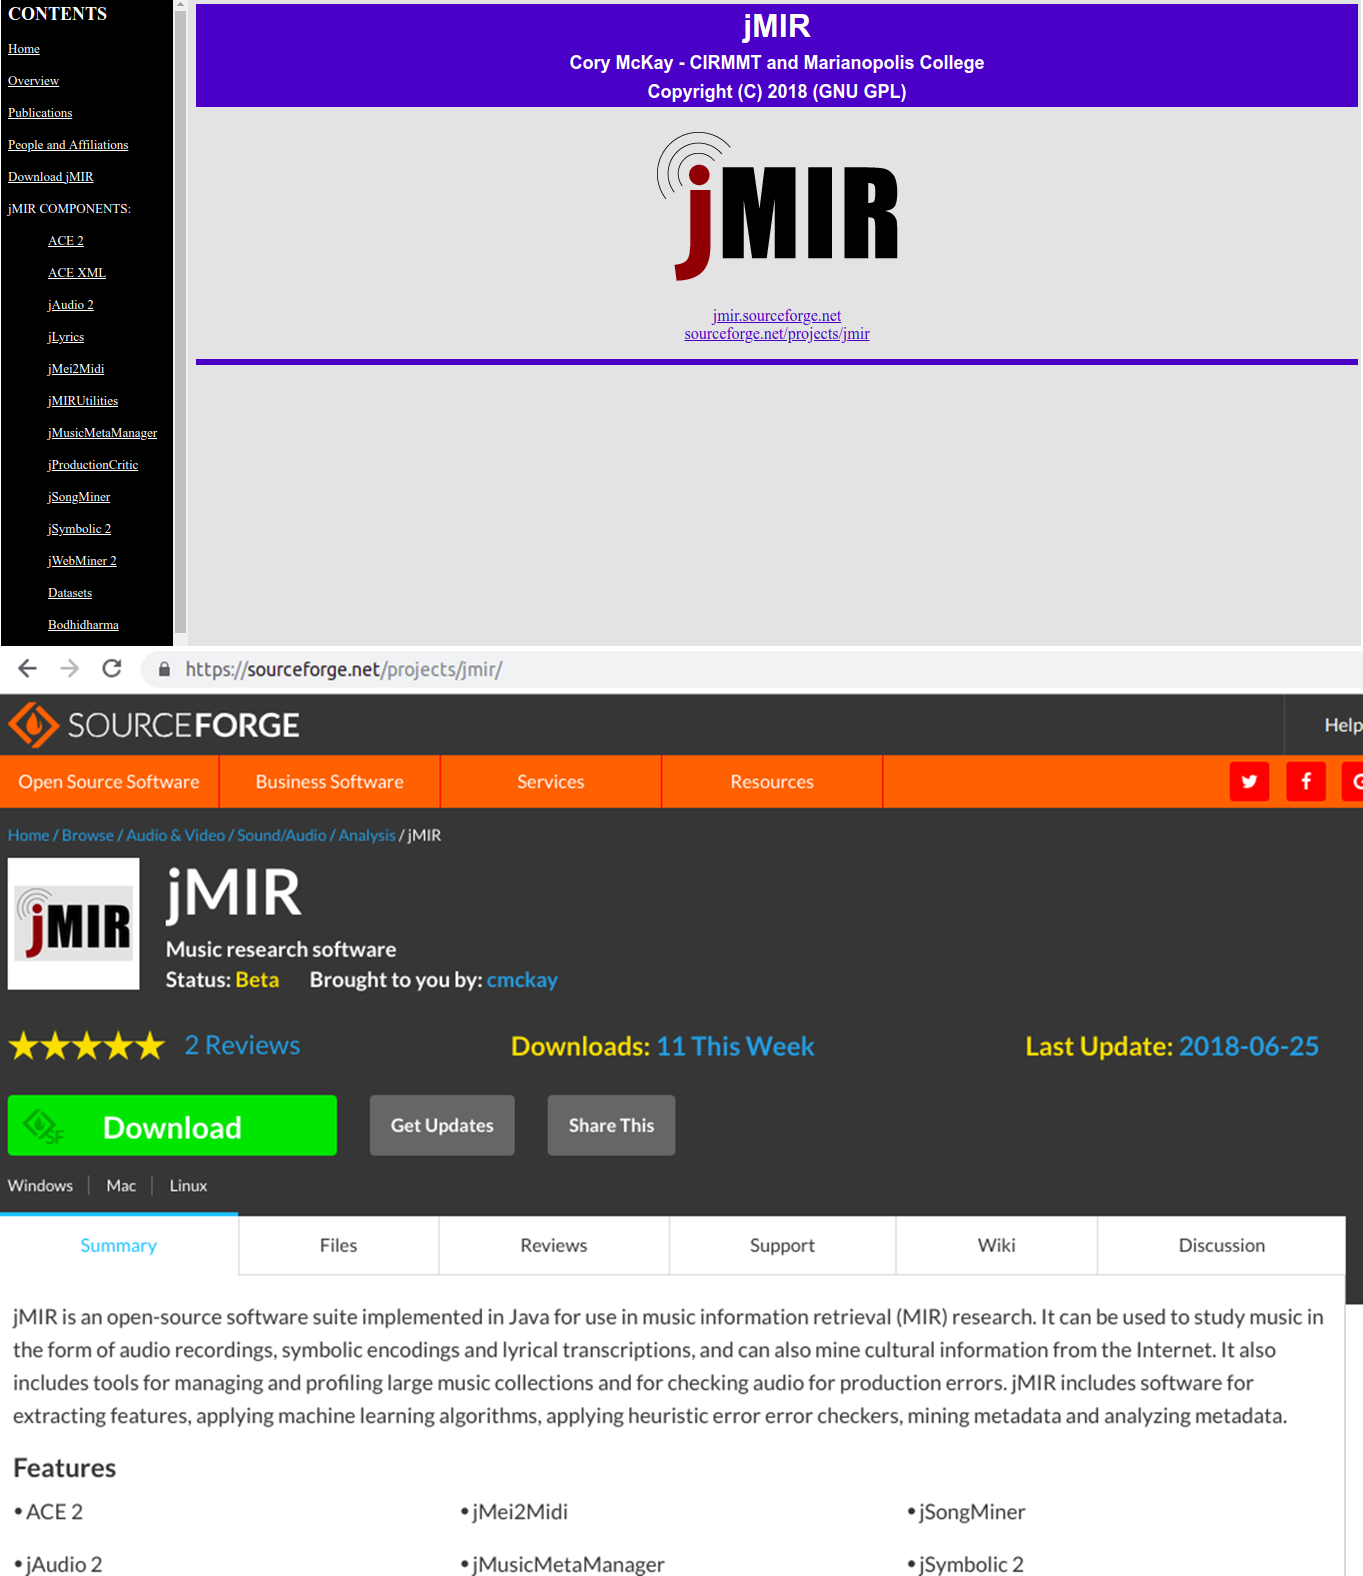
\includegraphics[scale=0.30]{figuras/jmir.png}
   \\Fonte: \cite{jmir}, elaborado pela autora
\end{figure}

\begin{figure}[!htb]
   \centering
   \caption{Tunebot}\label{fig:tunebot} 
   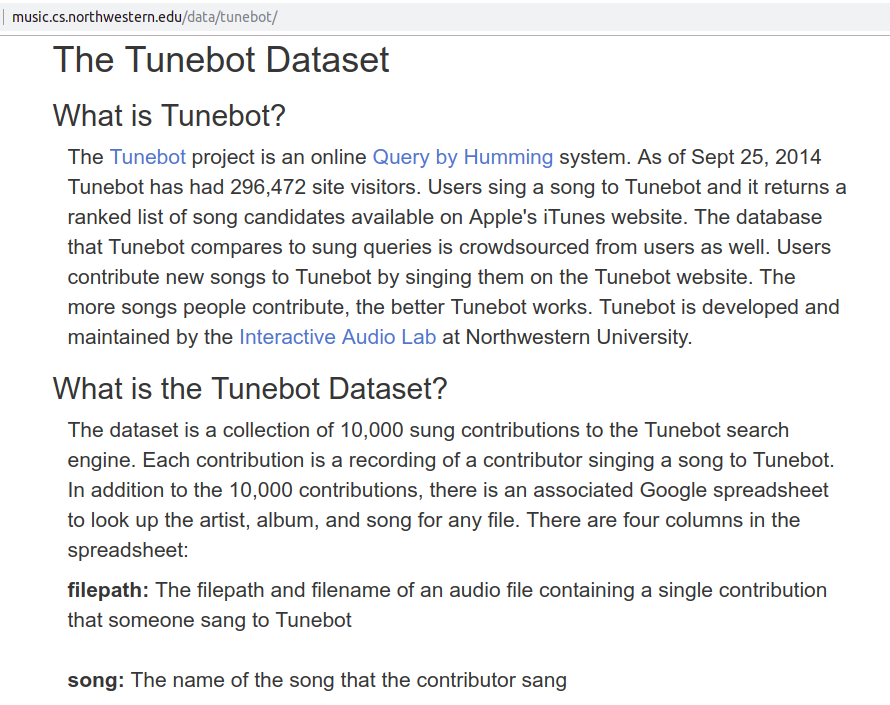
\includegraphics[scale=0.45]{figuras/tunebot.png}
   \\Fonte: \cite{tunebotiOS}, elaborado pela autora
\end{figure}

\begin{figure}[!htb]
   \centering
   \caption{CLAM}\label{fig:clam} 
   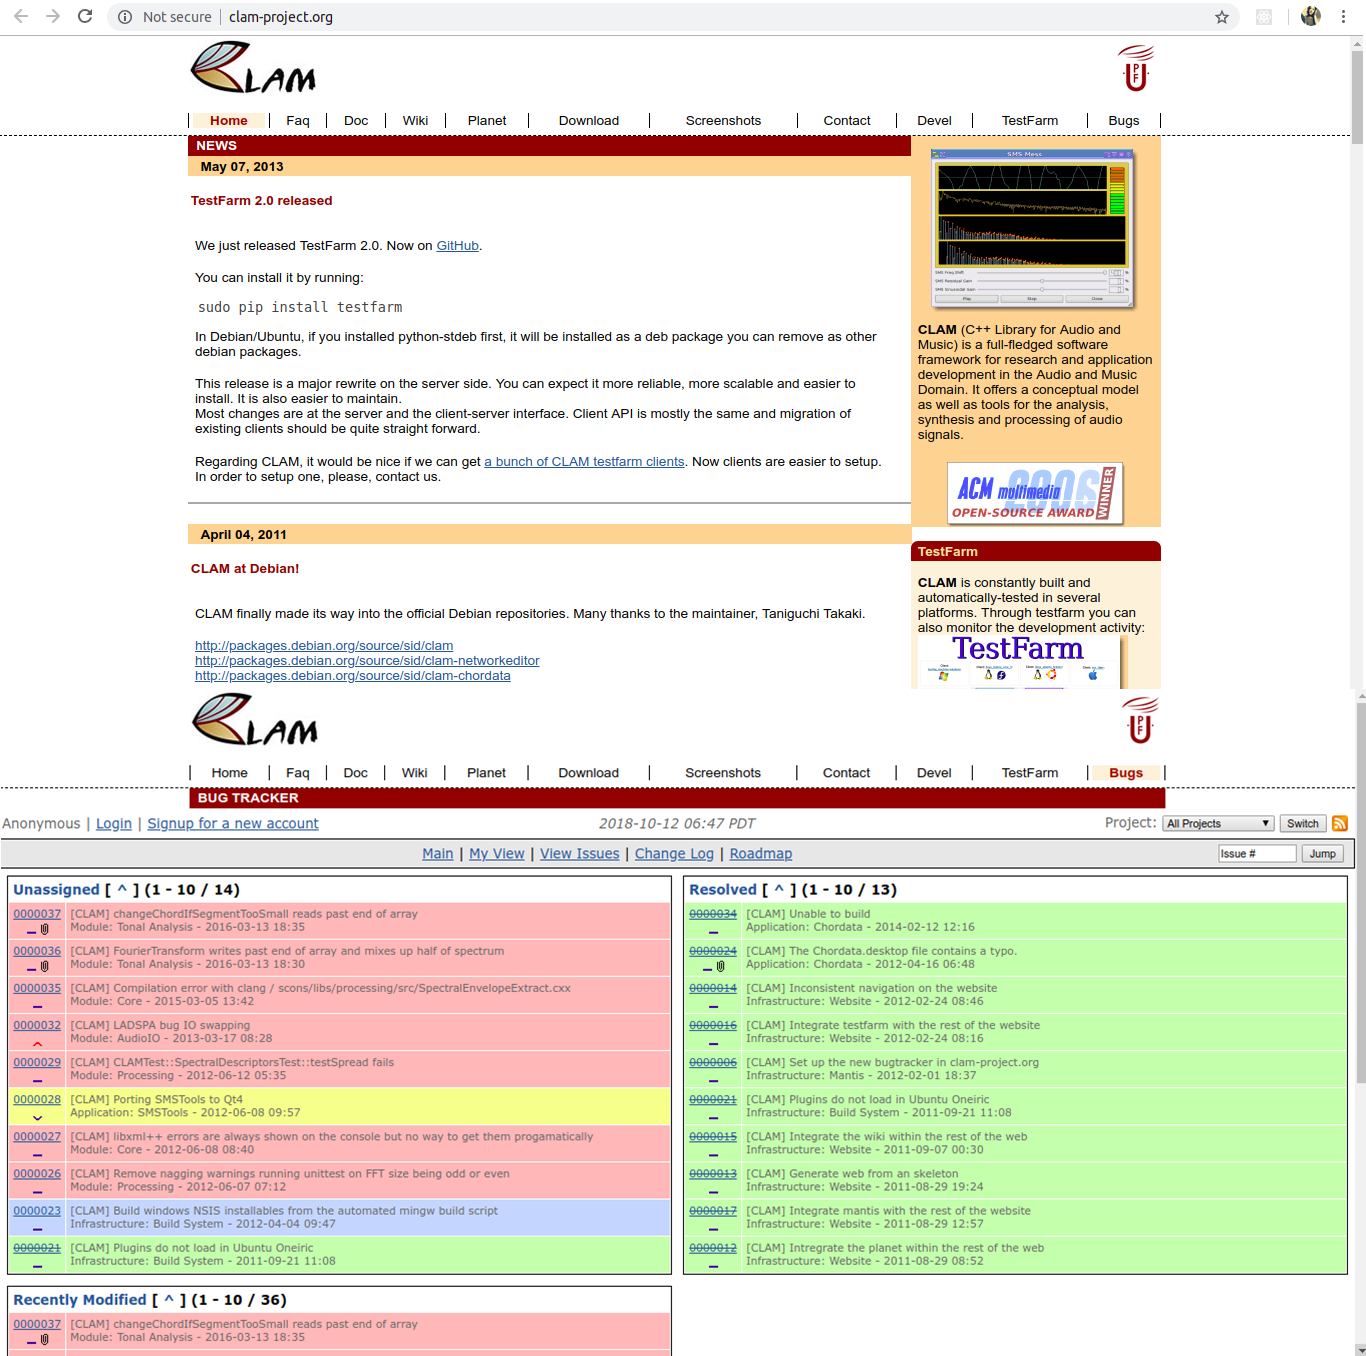
\includegraphics[scale=0.30]{figuras/clam.png}
   \\Fonte: \cite{clam}, elaborado pela autora
\end{figure}

\begin{figure}[!htb]
   \centering
   \caption{MIRtoolbox}\label{fig:mirtoolbox} 
   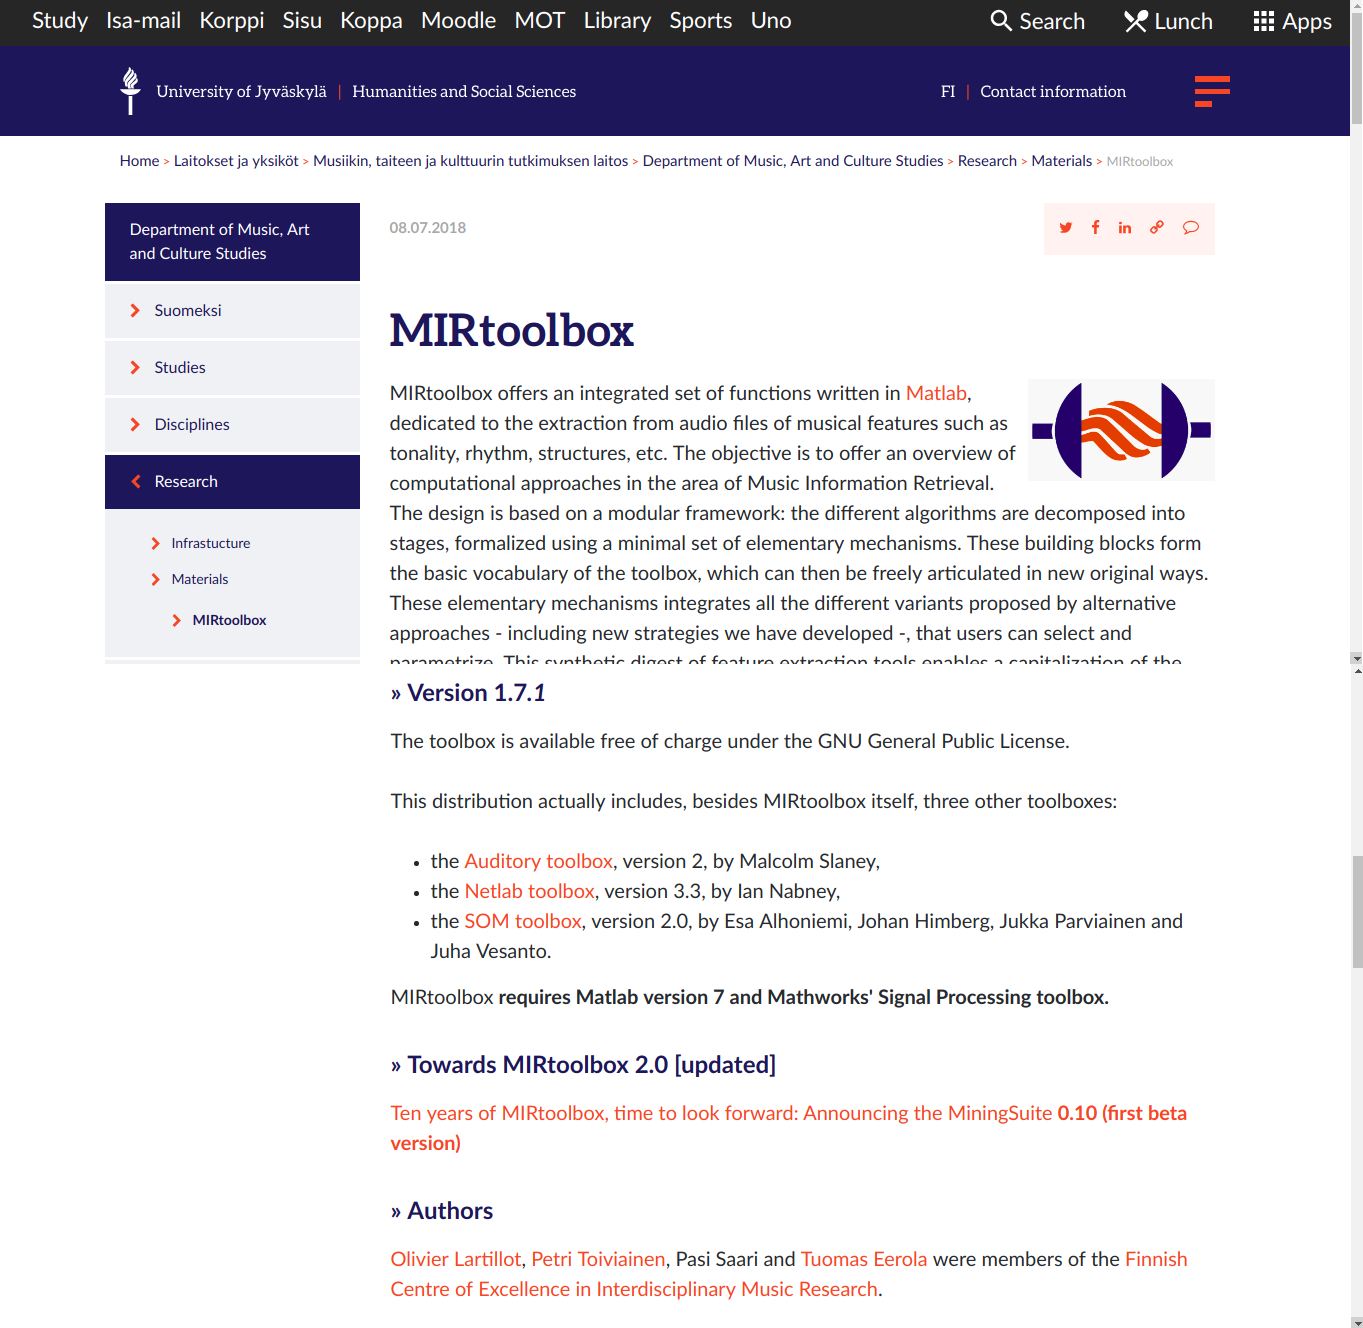
\includegraphics[scale=0.35]{figuras/mirtoolbox.png}
   \\Fonte: \cite{mirtoolbox}, elaborado pela autora
\end{figure}